%% DATACORE-X -- Health-aware economic MPC for data-centre cooling
%% Target: Applied Energy (Elsevier, elsarticle). Build: latexmk -pdf main.tex
\documentclass[preprint,12pt,authoryear]{elsarticle}
\usepackage{amsmath,amssymb}
\usepackage{booktabs}
\usepackage{adjustbox}
\usepackage{array}
\usepackage{graphicx}
\usepackage{siunitx}
\usepackage{xcolor}
\usepackage{hyperref}
\usepackage{lineno}
\usepackage[nameinlink]{cleveref}
\sisetup{detect-all}
\graphicspath{{figures/}}
% generated by dcx_paper_macros.m on 12-Nov-2026 22:08:48 -- do not edit
\newcommand{\CredItPeakInlet}{0.34}
\newcommand{\CredItRecover}{1}
\newcommand{\CredRecircPct}{8.6}
\newcommand{\CredRoomClosed}{0.01}
\newcommand{\CredRoomRaw}{-9.2}
\newcommand{\CredSettleChws}{4}
\newcommand{\CredSettleSat}{1.7}
\newcommand{\EfiveCrah}{0.983}
\newcommand{\EfiveCrahHi}{1.000}
\newcommand{\EfiveCrahLo}{0.931}
\newcommand{\EfiveCrahSensor}{0.955}
\newcommand{\EfivePlant}{0.988}
\newcommand{\EfivePlantHi}{1.000}
\newcommand{\EfivePlantLo}{0.979}
\newcommand{\EfivePlantSensor}{0.608}
\newcommand{\EfivePump}{1.000}
\newcommand{\EfivePumpHi}{1.000}
\newcommand{\EfivePumpLo}{1.000}
\newcommand{\EfivePumpSensor}{0.993}
\newcommand{\EfiveRulCover}{0.97}
\newcommand{\EfiveRulLate}{13.5}
\newcommand{\EfiveRulRmse}{18.5}
\newcommand{\EfiveRulRmseHi}{20.8}
\newcommand{\EfiveRulRmseLo}{17.3}
\newcommand{\EfiveRulRuns}{4}
\newcommand{\EfourSummary}{\Cref{tab:E4} and \cref{fig:E34} (right) report the effect of RUL error. chiller fault: trip rate 0.00/0.00/0.00/0.00/0.00 at RUL errors of -50/+0/+50/+100/+200\,\%; pump fault: trip rate 0.00/0.00/0.00/0.00/0.00 at RUL errors of -50/+0/+50/+100/+200\,\%.}
\newcommand{\EoneCoolPEmpcFixedAll}{<0.001}
\newcommand{\EoneCoolPEmpcFixedFrankfurt}{<0.001}
\newcommand{\EoneCoolPEmpcFixedPune}{<0.001}
\newcommand{\EoneCoolPHaEmpcAll}{<0.001}
\newcommand{\EoneCoolPHaEmpcFrankfurt}{0.002}
\newcommand{\EoneCoolPHaEmpcPune}{<0.001}
\newcommand{\EoneCoolPHaFixedAll}{<0.001}
\newcommand{\EoneCoolPHaFixedFrankfurt}{<0.001}
\newcommand{\EoneCoolPHaFixedPune}{<0.001}
\newcommand{\EoneCoolRelEmpcFixedAll}{-18.8}
\newcommand{\EoneCoolRelEmpcFixedAllHi}{-15.5}
\newcommand{\EoneCoolRelEmpcFixedAllLo}{-22.1}
\newcommand{\EoneCoolRelEmpcFixedFrankfurt}{-15.7}
\newcommand{\EoneCoolRelEmpcFixedFrankfurtHi}{-8.0}
\newcommand{\EoneCoolRelEmpcFixedFrankfurtLo}{-23.5}
\newcommand{\EoneCoolRelEmpcFixedPune}{-20.4}
\newcommand{\EoneCoolRelEmpcFixedPuneHi}{-20.0}
\newcommand{\EoneCoolRelEmpcFixedPuneLo}{-20.8}
\newcommand{\EoneCoolRelHaEmpcAll}{0.0}
\newcommand{\EoneCoolRelHaEmpcAllHi}{0.0}
\newcommand{\EoneCoolRelHaEmpcAllLo}{0.0}
\newcommand{\EoneCoolRelHaEmpcFrankfurt}{0.0}
\newcommand{\EoneCoolRelHaEmpcFrankfurtHi}{0.0}
\newcommand{\EoneCoolRelHaEmpcFrankfurtLo}{-0.0}
\newcommand{\EoneCoolRelHaEmpcPune}{0.0}
\newcommand{\EoneCoolRelHaEmpcPuneHi}{0.0}
\newcommand{\EoneCoolRelHaEmpcPuneLo}{0.0}
\newcommand{\EoneCoolRelHaFixedAll}{-18.8}
\newcommand{\EoneCoolRelHaFixedAllHi}{-15.5}
\newcommand{\EoneCoolRelHaFixedAllLo}{-22.1}
\newcommand{\EoneCoolRelHaFixedFrankfurt}{-15.7}
\newcommand{\EoneCoolRelHaFixedFrankfurtHi}{-8.0}
\newcommand{\EoneCoolRelHaFixedFrankfurtLo}{-23.5}
\newcommand{\EoneCoolRelHaFixedPune}{-20.4}
\newcommand{\EoneCoolRelHaFixedPuneHi}{-19.9}
\newcommand{\EoneCoolRelHaFixedPuneLo}{-20.8}
\newcommand{\EoneFacPEmpcFixedAll}{<0.001}
\newcommand{\EoneFacPEmpcFixedFrankfurt}{<0.001}
\newcommand{\EoneFacPEmpcFixedPune}{<0.001}
\newcommand{\EoneFacPHaEmpcAll}{<0.001}
\newcommand{\EoneFacPHaEmpcFrankfurt}{0.030}
\newcommand{\EoneFacPHaEmpcPune}{<0.001}
\newcommand{\EoneFacPHaFixedAll}{<0.001}
\newcommand{\EoneFacPHaFixedFrankfurt}{<0.001}
\newcommand{\EoneFacPHaFixedPune}{<0.001}
\newcommand{\EoneFacRelEmpcFixedAll}{-2.3}
\newcommand{\EoneFacRelEmpcFixedAllHi}{-1.9}
\newcommand{\EoneFacRelEmpcFixedAllLo}{-2.7}
\newcommand{\EoneFacRelEmpcFixedFrankfurt}{-1.3}
\newcommand{\EoneFacRelEmpcFixedFrankfurtHi}{-0.7}
\newcommand{\EoneFacRelEmpcFixedFrankfurtLo}{-2.0}
\newcommand{\EoneFacRelEmpcFixedPune}{-3.2}
\newcommand{\EoneFacRelEmpcFixedPuneHi}{-3.1}
\newcommand{\EoneFacRelEmpcFixedPuneLo}{-3.3}
\newcommand{\EoneFacRelHaEmpcAll}{0.0}
\newcommand{\EoneFacRelHaEmpcAllHi}{0.0}
\newcommand{\EoneFacRelHaEmpcAllLo}{0.0}
\newcommand{\EoneFacRelHaEmpcFrankfurt}{0.0}
\newcommand{\EoneFacRelHaEmpcFrankfurtHi}{0.0}
\newcommand{\EoneFacRelHaEmpcFrankfurtLo}{-0.0}
\newcommand{\EoneFacRelHaEmpcPune}{0.0}
\newcommand{\EoneFacRelHaEmpcPuneHi}{0.0}
\newcommand{\EoneFacRelHaEmpcPuneLo}{0.0}
\newcommand{\EoneFacRelHaFixedAll}{-2.3}
\newcommand{\EoneFacRelHaFixedAllHi}{-1.9}
\newcommand{\EoneFacRelHaFixedAllLo}{-2.7}
\newcommand{\EoneFacRelHaFixedFrankfurt}{-1.3}
\newcommand{\EoneFacRelHaFixedFrankfurtHi}{-0.7}
\newcommand{\EoneFacRelHaFixedFrankfurtLo}{-2.0}
\newcommand{\EoneFacRelHaFixedPune}{-3.2}
\newcommand{\EoneFacRelHaFixedPuneHi}{-3.1}
\newcommand{\EoneFacRelHaFixedPuneLo}{-3.3}
\newcommand{\EonePueEmpcFrankfurt}{1.192}
\newcommand{\EonePueEmpcPune}{1.269}
\newcommand{\EonePueFixedFrankfurt}{1.208}
\newcommand{\EonePueFixedPune}{1.311}
\newcommand{\EonePueHaFrankfurt}{1.192}
\newcommand{\EonePueHaPune}{1.269}
\newcommand{\EonePuePEmpcFixedAll}{<0.001}
\newcommand{\EonePuePEmpcFixedFrankfurt}{<0.001}
\newcommand{\EonePuePEmpcFixedPune}{<0.001}
\newcommand{\EonePuePHaEmpcAll}{<0.001}
\newcommand{\EonePuePHaEmpcFrankfurt}{0.028}
\newcommand{\EonePuePHaEmpcPune}{<0.001}
\newcommand{\EonePuePHaFixedAll}{<0.001}
\newcommand{\EonePuePHaFixedFrankfurt}{<0.001}
\newcommand{\EonePuePHaFixedPune}{<0.001}
\newcommand{\EonePueRelEmpcFixedAll}{-2.3}
\newcommand{\EonePueRelEmpcFixedAllHi}{-1.9}
\newcommand{\EonePueRelEmpcFixedAllLo}{-2.7}
\newcommand{\EonePueRelEmpcFixedFrankfurt}{-1.3}
\newcommand{\EonePueRelEmpcFixedFrankfurtHi}{-0.7}
\newcommand{\EonePueRelEmpcFixedFrankfurtLo}{-2.0}
\newcommand{\EonePueRelEmpcFixedPune}{-3.2}
\newcommand{\EonePueRelEmpcFixedPuneHi}{-3.1}
\newcommand{\EonePueRelEmpcFixedPuneLo}{-3.3}
\newcommand{\EonePueRelHaEmpcAll}{0.0}
\newcommand{\EonePueRelHaEmpcAllHi}{0.0}
\newcommand{\EonePueRelHaEmpcAllLo}{0.0}
\newcommand{\EonePueRelHaEmpcFrankfurt}{0.0}
\newcommand{\EonePueRelHaEmpcFrankfurtHi}{0.0}
\newcommand{\EonePueRelHaEmpcFrankfurtLo}{-0.0}
\newcommand{\EonePueRelHaEmpcPune}{0.0}
\newcommand{\EonePueRelHaEmpcPuneHi}{0.0}
\newcommand{\EonePueRelHaEmpcPuneLo}{0.0}
\newcommand{\EonePueRelHaFixedAll}{-2.3}
\newcommand{\EonePueRelHaFixedAllHi}{-1.9}
\newcommand{\EonePueRelHaFixedAllLo}{-2.7}
\newcommand{\EonePueRelHaFixedFrankfurt}{-1.3}
\newcommand{\EonePueRelHaFixedFrankfurtHi}{-0.7}
\newcommand{\EonePueRelHaFixedFrankfurtLo}{-2.0}
\newcommand{\EonePueRelHaFixedPune}{-3.2}
\newcommand{\EonePueRelHaFixedPuneHi}{-3.1}
\newcommand{\EonePueRelHaFixedPuneLo}{-3.3}
\newcommand{\EoneTtwentyEightEmpcFrankfurt}{0.0}
\newcommand{\EoneTtwentyEightEmpcPune}{0.0}
\newcommand{\EoneTtwentyEightFixedFrankfurt}{0.0}
\newcommand{\EoneTtwentyEightFixedPune}{0.0}
\newcommand{\EoneTtwentyEightHaFrankfurt}{0.0}
\newcommand{\EoneTtwentyEightHaPune}{0.0}
\newcommand{\EsixMaxMs}{903}
\newcommand{\EsixMeanMs}{25}
\newcommand{\EthreeSummary}{Across both fault scenarios and climates: the full controller: 0/40 unplanned trips, 12.2\,min zone-C/D exposure, peak inlet 26.60\,\textdegree C; removing the HI: 3/40 unplanned trips, 17.4\,min zone-C/D exposure, peak inlet 26.62\,\textdegree C; removing RUL: 1/40 unplanned trips, 12.2\,min zone-C/D exposure, peak inlet 26.60\,\textdegree C; removing pre-cooling: 1/40 unplanned trips, 12.2\,min zone-C/D exposure, peak inlet 26.60\,\textdegree C; health-blind EMPC: 34/40 unplanned trips, 25.1\,min zone-C/D exposure, peak inlet 26.67\,\textdegree C.}
\newcommand{\EtwoEnergyRelHaEmpc}{-0.0}
\newcommand{\EtwoEnergyRelHaEmpcHi}{-0.0}
\newcommand{\EtwoEnergyRelHaEmpcLo}{-0.0}
\newcommand{\EtwoRiskEmpc}{50.3}
\newcommand{\EtwoRiskFixed}{49.8}
\newcommand{\EtwoRiskHa}{24.5}
\newcommand{\EtwoTripsEmpc}{34/40}
\newcommand{\EtwoTripsFixed}{37/40}
\newcommand{\EtwoTripsHa}{0/40}
\newcommand{\cpuHours}{3}
\newcommand{\nRuns}{586}


\journal{Applied Energy}

\begin{document}
\begin{frontmatter}

\title{Health-aware economic model predictive control of data-centre cooling using live equipment Health Index and remaining-useful-life estimates: a verified multi-climate simulation study}

\author[vit]{Anup Deshmukh\corref{cor1}}
\ead{TODO@example.com}
\cortext[cor1]{Corresponding author.}
\address[vit]{Department of Instrumentation and Control Engineering, Vishwakarma Institute of Technology, Pune, India}

\begin{abstract}
Economic model predictive control (EMPC) can lower the energy used to cool data centres, but published designs assume that chillers, pumps and fans stay healthy, so degradation is handled separately, after a fault is detected.
We propose PI-HA-EMPC, a supervisory EMPC that consumes a live Health Index (HI) and remaining-useful-life (RUL) estimate of the cooling equipment, both computed online from measured signals with physics residuals.
Health enters the controller in three ways: health-scaled move bounds on the supervisory setpoints, RUL-triggered pre-cooling, and prognostic discrete actions (pump changeover, standby-chiller pre-start and lead transfer).
The method is evaluated on a calibrated, cross-verified simulation twin of an 8-rack air-cooled facility in two climates (Pune, India; Frankfurt, Germany), three IT-workload profiles and ten seeds spread across the year (\nRuns{} closed-loop runs).
In normal operation PI-HA-EMPC changed cooling energy by \EoneCoolRelHaFixedPune\,\% (95\,\% CI \EoneCoolRelHaFixedPuneLo{} to \EoneCoolRelHaFixedPuneHi\,\%) in Pune and \EoneCoolRelHaFixedFrankfurt\,\% (\EoneCoolRelHaFixedFrankfurtLo{} to \EoneCoolRelHaFixedFrankfurtHi\,\%) in Frankfurt relative to fixed-setpoint control, with no time above the 28\,\textdegree C inlet limit, while its energy use stayed within 0.05\,\% of health-blind EMPC in every paired run.
Under chiller and pump degradation leading to protective trips, unplanned trips fell from \EtwoTripsEmpc{} with EMPC to \EtwoTripsHa{} with PI-HA-EMPC.
Component ablations show that the benefit comes from the health-triggered discrete actions: health used only inside the MPC (move bounds and pre-cooling) avoided none of the trips, whereas the discrete actions alone avoided all of them. The HI and RUL triggers back each other up, so the scheme tolerated RUL over-estimates of up to $3\times$ without additional trips.
A co-simulation with a Simscape Fluids model of the chilled-water network in the closed loop reproduced the reduced-order results for the pump-fault scenario.
The mean MPC solve time was \EsixMeanMs\,ms per 60\,s step.
All results are from simulation; models, configuration and seeds are released for reproduction.
\end{abstract}

\begin{highlights}
\item Economic MPC for data-centre cooling that uses live Health Index and RUL.
\item Health-scaled move bounds, RUL-triggered pre-cooling and prognostic actions.
\item 500 seeded runs across two climates, three workloads and ten days of the year.
\item Unplanned trips avoided at no measurable energy cost; HI and RUL triggers are redundant.
\item Verified, calibrated open simulation twin; simulation-only results.
\end{highlights}

\begin{keyword}
data centre cooling \sep economic model predictive control \sep health-aware control \sep remaining useful life \sep predictive maintenance \sep digital twin
\end{keyword}
\end{frontmatter}

\linenumbers

%% =====================================================================
\section{Introduction}\label{sec:intro}
Cooling is the largest non-IT energy use in most air-cooled data centres, and it must keep IT inlet air inside the ASHRAE envelope \citep{ASHRAETC99}. Supervisory model predictive control (MPC) is an established way to cut this energy by co-optimising chilled-water and air-side setpoints against forecast IT load and weather \citep{Lazic2018,Fan2023WSE,Boldocky2026MIDPC}. Recent digital-twin studies go further and quantify how much of the theoretically optimal saving survives practical constraints: \citet{Jadhav2026DT} introduce an \emph{implementability gap} and show that actuator ramp-rate limits retain 27.8\,\% of a 30.1\,\% theoretical saving on the Frontier liquid-cooling system, and \citet{Zhang2026DCVerse} vet reinforcement-learning policies on a twin before deployment.

These works share an assumption: the chillers, pumps and fans are healthy, or their faults are handled after detection by a separate fault-tolerant layer \citep{Kheradmandi2020FTC}. In operation, however, cooling equipment degrades gradually: bearings wear, chillers lose capacity and efficiency, and heat exchangers foul. Each of these eventually ends in a protective trip, and each trip forces a thermal transient. Health-aware control, which feeds prognostic information into the controller, is well established in water networks \citep{Grosso2016RBEMPC}, wind turbines \citep{Sanchez2017HAMPC}, process plants \citep{Matias2025HAC} and hydraulic actuators \citep{Kaki2026EHA}, building on \citet{Escobet2012HAC} and reliability-based RUL assessment \citep{KarimiPour2018LPV}. To our knowledge it has not been formulated for, or evaluated on, the supervisory control of a data-centre cooling plant, where degradation of one asset is coupled to the thermal safety of the whole IT load.

\paragraph{Gap} Existing data-centre cooling optimisation, including the implementability-gap work, quantifies the cost of \emph{actuator} constraints but not of \emph{equipment condition}. No study we found (i) feeds live HI and RUL estimates of the cooling equipment into an economic supervisory controller, (ii) measures the trade-off between energy and avoided unplanned trips with statistical confidence across climates and workloads, or (iii) tests how sensitive such a controller is to RUL estimation error.

\paragraph{Contributions}
\begin{enumerate}
\item \textbf{PI-HA-EMPC} (\cref{sec:method}): an EMPC that consumes online HI and RUL through three mechanisms: health-scaled move bounds, RUL-triggered pre-cooling, and prognostic discrete actions (pump changeover; standby-chiller pre-start followed by lead transfer).
\item \textbf{An evaluation protocol} (\cref{sec:design}) with experiments E1--E6: two climates, three workload profiles, ten seeds spread over the year, paired statistics with 95\,\% confidence intervals, ablations of each health mechanism, sensitivity to RUL estimation error, and MPC solve time.
\item \textbf{Credibility evidence} (\cref{sec:cred}): energy-balance closure, step responses, calibration against ASHRAE 90.1 and measured weather, validation of the hydraulics against Simscape Fluids, both open-loop and with the Simscape network in the closed loop, and cross-verification of two independent implementations.
\end{enumerate}
The 3D digital twin and SCADA (OPC~UA/Ignition) integration used to build and operate the testbed are enabling infrastructure and are not claimed as contributions. All results are from simulation.

%% =====================================================================
\section{Related work}\label{sec:related}
\Cref{tab:related} positions this work. MPC and EMPC for chiller plants and data centres optimise energy or cost under thermal constraints \citep{Lazic2018,Fan2023WSE,Satue2025EMPC,Boldocky2026MIDPC,Kim2020RTU}. Digital-twin optimisation studies add validation against operational data and implementability analysis \citep{Jadhav2026DT,Jadhav2026CoDesign,Zhang2026DCVerse}. Fault-tolerant data-centre control reconfigures after a sensor or actuator fault has been detected \citep{Kheradmandi2020FTC}. Health-aware MPC trades performance against degradation using prognostics \citep{Escobet2012HAC,Grosso2016RBEMPC,KarimiPour2018LPV,Sanchez2017HAMPC,Matias2025HAC,Kaki2026EHA}, but in domains whose degradation mechanisms and safety constraints differ from those of a cooling plant serving IT load.

\begin{table}[t]\centering\small
\caption{Positioning against representative work. \checkmark: addressed; --: not addressed.}\label{tab:related}
\begin{adjustbox}{max width=\linewidth}\begin{tabular}{lccccc}
\toprule
Work & DC & Economic & Online HI/RUL & Prognostic & Multi-climate\\
 & cooling & MPC & in control & actions & statistics\\
\midrule
\citet{Lazic2018} & \checkmark & \checkmark & -- & -- & --\\
\citet{Fan2023WSE} & \checkmark & \checkmark & -- & -- & --\\
\citet{Jadhav2026DT} & \checkmark & (optimiser) & -- & -- & --\\
\citet{Zhang2026DCVerse} & \checkmark & (DRL) & -- & -- & --\\
\citet{Kheradmandi2020FTC} & \checkmark & \checkmark & -- (post-detection) & -- & --\\
\citet{Grosso2016RBEMPC} & -- & \checkmark & \checkmark & -- & --\\
\citet{Matias2025HAC} & -- & \checkmark & \checkmark & -- & --\\
This work & \checkmark & \checkmark & \checkmark & \checkmark & \checkmark\\
\bottomrule
\end{tabular}\end{adjustbox}
\end{table}

%% =====================================================================
\section{Testbed}\label{sec:testbed}
The reference facility is a hypothetical 8-rack, roughly 100\,kW air-cooled data hall with contained cold aisle, four CRAH units, a chilled-water (CHW) loop with three parallel variable-speed pumps (duty/standby), a water-side economiser heat exchanger, two water-cooled chillers (lead/lag with 180\,s start-up delay), two cooling towers, and a 2N UPS electrical path with generator and ATS. The plant is a reduced-order, fixed-step (1\,s) model implemented twice: as a Simulink model with Stateflow sequencing of the generator and ATS, and as a MATLAB reference stepper. Each is cross-verified against an independent Python surrogate (\cref{sec:cred}). Rack thermals are lumped RC models; CRAH coils use effectiveness--NTU; hydraulics solve parallel pump curves against a valve-dependent system curve; chillers follow a Carnot-fraction map with part-load correction; towers use an approach model. Sensors add noise, quantisation and drift to 217 measured points. Faults (21 types) ramp from incipient to severe and end in protective trips at physically motivated thresholds (e.g.\ ISO 10816 zone D vibration \citep{ISO10816}).

Calibration (\cref{tab:calib}) fixes the chiller map to the ASHRAE 90.1 minimum ratings \citep{ASHRAE901}, the tower fan to the 90.1 minimum tower efficiency, and the CHW system curve to a Simscape Fluids network. Ambient conditions use measured 2025 hourly weather for Pune and Frankfurt \citep{Hersbach2020ERA5}, with wet bulb computed after \citet{Stull2011}. Carbon accounting uses the Indian CEA v20.0 grid factor of 0.727\,kg/kWh \citep{CEA2024} and the 2024 German factor of 0.363\,kg/kWh \citep{UBA2025}.

\begin{table}[t]\centering\small
\caption{Calibration of the plant (calibrated profile).}\label{tab:calib}
\begin{tabular}{>{\raggedright}p{0.17\linewidth}>{\raggedright}p{0.38\linewidth}>{\raggedright\arraybackslash}p{0.37\linewidth}}
\toprule
Item & Reference & Result\\
\midrule
Chiller map & ASHRAE 90.1 Tab.\ 6.8.1-3 (FL 0.750, IPLV 0.600\,kW/ton) & $\eta_c=0.511$, part-load $a=0.552$; both ratings reproduced\\
Tower fan & ASHRAE 90.1 Tab.\ 6.8.1-7 ($\ge$40.2\,gpm/hp) & 3.53\,kW (was 5.5\,kW, below minimum)\\
CHW pumping & 90.1 App.\ G (22\,W/gpm) & 22.0\,W/gpm at design flow\\
CHW system curve & Simscape Fluids network, 41 points & $\Delta p-H_s=(1.62+4.36/v^2)q^2$; RMS flow error 1.6\,\%\\
Weather & ERA5 (Open-Meteo), 2025 & Pune wet bulb mean 19.2\,\textdegree C; Frankfurt 8.3\,\textdegree C\\
Grid factor & CEA v20.0; UBA 2025 & 0.727 / 0.363 kg\,CO$_2$/kWh\\
\bottomrule
\end{tabular}
\end{table}

%% =====================================================================
\section{Method}\label{sec:method}
\subsection{Online health estimation}
Health is computed every 60\,s from \emph{measured} signals only; the controller has no access to the injected faults. For CHW pump $i$ running at normalised speed $n_i$, the vibration residual against the healthy speed-dependent baseline is
\begin{equation}
r_{v,i}=v_i-(0.9+1.3\,n_i^2),\qquad \mathrm{HI}_{p,i}=100\,\bigl(1-\mathrm{sat}_{[0,1]}(r_{v,i}/5.45)\bigr),
\end{equation}
where 5.45\,mm/s is the residual at which the pump reaches the ISO 10816 zone-D trip level. For the lead chiller, the relative COP residual against the calibrated performance map evaluated at the measured part load and condenser-water temperature is $r_c=(\mathrm{COP}_{\mathrm{map}}-\mathrm{COP})/\mathrm{COP}_{\mathrm{map}}$, and $\mathrm{HI}_c=100(1-\mathrm{sat}_{[0,1]}(2.2\,r_c))$. RUL is the time for a degradation signal to reach its threshold, extrapolated from a linear trend over the last 15 samples:
\begin{equation}
\widehat{\mathrm{RUL}}=\frac{\theta-\hat\beta_0}{\hat\beta_1}\quad(\hat\beta_1>0),\qquad \widehat{\mathrm{RUL}}=\infty\ \text{otherwise}.
\end{equation}
The separate offline diagnosis and prognosis pipeline (bagged trees on sensor and physics-residual features; exponential and linear degradation models) is evaluated in E5.

\subsection{Economic MPC}
The supervisory layer acts every $T_s=60$\,s on three manipulated variables, $u=[T_{\mathrm{chws}}^{\mathrm{sp}},\,T_{\mathrm{sa}}^{\mathrm{sp}},\,T_{\mathrm{in,max}}^{\mathrm{sp}}]$: the CHW supply, supply-air and maximum-inlet setpoints, which are tracked by the plant's PI loops. Measured disturbances are the IT load and the wet bulb; the outputs are the maximum rack inlet temperature $y_1$ and the facility power $y_2$. A discrete state-space prediction model is identified for each climate by \texttt{ssest}/\texttt{n4sid} from 48\,h of excitation spread over four seasons, with order selected on held-out data. The fit on held-out data is 81.8\,\% (inlet) and 66.5\,\% (power) for Pune, and 81.3\,\% and 55.3\,\% for Frankfurt. The EMPC solves
\begin{equation}
\begin{aligned}
&\min_{\Delta u}\ \sum_{k=1}^{N_p}\bigl(y_{2,k}-y_2^{\mathrm{ref}}\bigr)^2+\rho_\epsilon\epsilon^2+\sum_{k=0}^{N_c-1}\Delta u_k^{\top}W\Delta u_k\\
&\ \text{s.t.}\ \ y_{1,k}\le \bar T-\delta+\epsilon,\quad \underline u\le u_k\le\bar u,\quad |\Delta u_k|\le r,
\end{aligned}
\end{equation}
with $y_2^{\mathrm{ref}}$ far below any feasible power (economic objective), $N_p=20$, $N_c=4$, $\bar T=27$\,\textdegree C, a back-off of $\delta=0.2$\,K for model error, and a nominal slew rate of $r=0.5$\,K/min.

\subsection{Health-aware extensions (PI-HA-EMPC)}
\begin{enumerate}
\item \emph{Health-scaled move bounds}: $r\leftarrow g\,r$ with
\[g=\max\bigl(0.25,\ \min(\mathrm{HI}_c,\min_i\mathrm{HI}_{p,i})/100\bigr),\]
so the supervisor stops making aggressive setpoint moves that stress degraded equipment.
\item \emph{RUL-triggered pre-cooling}: if $\min\widehat{\mathrm{RUL}}<W_{\mathrm{RUL}}=25$\,min or $\mathrm{HI}_c<45$, the inlet limit is tightened to 24.5\,\textdegree C and the setpoint bounds are lowered, building thermal margin before a predicted failure.
\item \emph{Prognostic discrete actions}: a CHW pump changeover when the duty pump's $\widehat{\mathrm{RUL}}<15$\,min or $\mathrm{HI}<25$. For a degrading lead chiller, a standby-chiller pre-start (which absorbs the 180\,s start-up delay) followed after 240\,s by a lead transfer. The sequence is latched: once the pre-start is issued, the transfer follows even if the trigger drops out (\cref{sec:discussion}).
\end{enumerate}
The baselines are fixed setpoints with PI control (the ``thermostatic'' baseline) and the same EMPC without health information.

%% =====================================================================
\section{Experimental design}\label{sec:design}
Every run lasts 6\,h from 11:00 with a +20\,\% IT-load ramp over 2\,h. Seed $k\in\{1,\dots,10\}$ sets the utilisation noise and the start day $15+36(k-1)$, so the ten seeds sample weather across the year. Workloads are a diurnal swing, flat load, and bursty batch blocks (45\,min high / 45\,min low). Fault scenarios are \emph{chiller} (CH-01 degradation from 1\,h over 2\,h, protective trip at 3.2\,h) and \emph{pump} (P-01 bearing degradation from 0.5\,h over 2.5\,h, zone-D trip at 94\,\% of the ramp). A trip is \emph{unplanned} if the asset is still on duty when it trips.
\begin{description}
\item[E1] Energy and thermal performance in the normal scenario (2 climates $\times$ 3 workloads $\times$ 10 seeds $\times$ 3 controllers).
\item[E2] Equipment risk under faults: unplanned-trip rate (Wilson 95\,\% CI) and time a running pump spends in ISO 10816 zone C/D ($>$4.5\,mm/s).
\item[E3] Ablations: PI-HA-EMPC without HI, without RUL, and without pre-cooling.
\item[E4] Sensitivity to RUL estimation error: every RUL estimate multiplied by $0.5$, $1.5$, $2.0$ or $3.0$ (pessimistic $-50$\,\% to optimistic $+200$\,\%; the unscaled case is the E2 run).
\item[E5] Diagnosis macro-F1 and RUL error of the offline predictive-maintenance pipeline.
\item[E6] Computational cost: \texttt{mpcmove} wall time per step.
\end{description}
Metrics are cooling and facility energy, energy-weighted PUE, CO$_2$, time above 27 and 28\,\textdegree C, peak inlet, unplanned trips and zone-C/D exposure. Controllers are compared \emph{paired} on identical seed, climate and workload. We report the mean difference with a 95\,\% $t$-interval and a Wilcoxon signed-rank $p$-value.

%% =====================================================================
\section{Model credibility}\label{sec:cred}
\paragraph{Cross-verification} The Simulink model and the MATLAB reference stepper each match an independent Python implementation on 42/42 checks (6 scenarios $\times$ 7 signals). A further 670 physics and scenario checks on the twin's published values all pass. These include closure of rack, coil and plant heat balances, pump power $=qH/\eta$, chiller power $=Q/\mathrm{COP}$ and PUE.
\paragraph{Simscape Fluids in the closed loop} To check that the controller results do not depend on the reduced-order hydraulics, the Simscape Fluids (Isothermal Liquid) model of the CHW network (two centrifugal pump trains, isolation valves, four CRAH branches with pipes, coils and control valves) was co-simulated with the plant. Every 10\,s the network is advanced from its saved operating point with the plant's VFD speed, pump run states and valve openings. Its header differential pressure and loop and per-pump flows then replace the reduced-order hydraulics: the DP loop regulates on the Simscape pressure, the coils transfer heat with the Simscape flow, and pump power is recomputed from the Simscape flows. The supervisor's changeover reaches the network through the pump run states. For the pump-bearing scenario (Pune, seed 1, 6\,h) with PI-HA-EMPC and with EMPC (\cref{fig:sscloop}), outcomes were unchanged: no trip with PI-HA-EMPC, and a trip at 2.85\,h with EMPC in both models. The DP held its setpoint in both models, mean loop flow differed by 0.1\,\% and facility energy by less than 0.01\,\%. The models differ in the pump-switch transient. When the faulty pump trips, the Simscape flow dips to 4.32\,L/s against 4.66\,L/s in the reduced model, which lags the flow with a first-order filter. The planned changeover is bumpless in both. With Simscape the PI-HA-EMPC changeover came 4\,min earlier (2.38\,h against 2.45\,h). The same shift occurs in the reduced model when its flow is scaled by $1.001$, so it reflects the sensitivity of the changeover trigger to small perturbations ($\pm$5\,min for $\pm$0.1--0.2\,\% flow), not a disagreement between the hydraulic models.
\begin{figure}[t]\centering
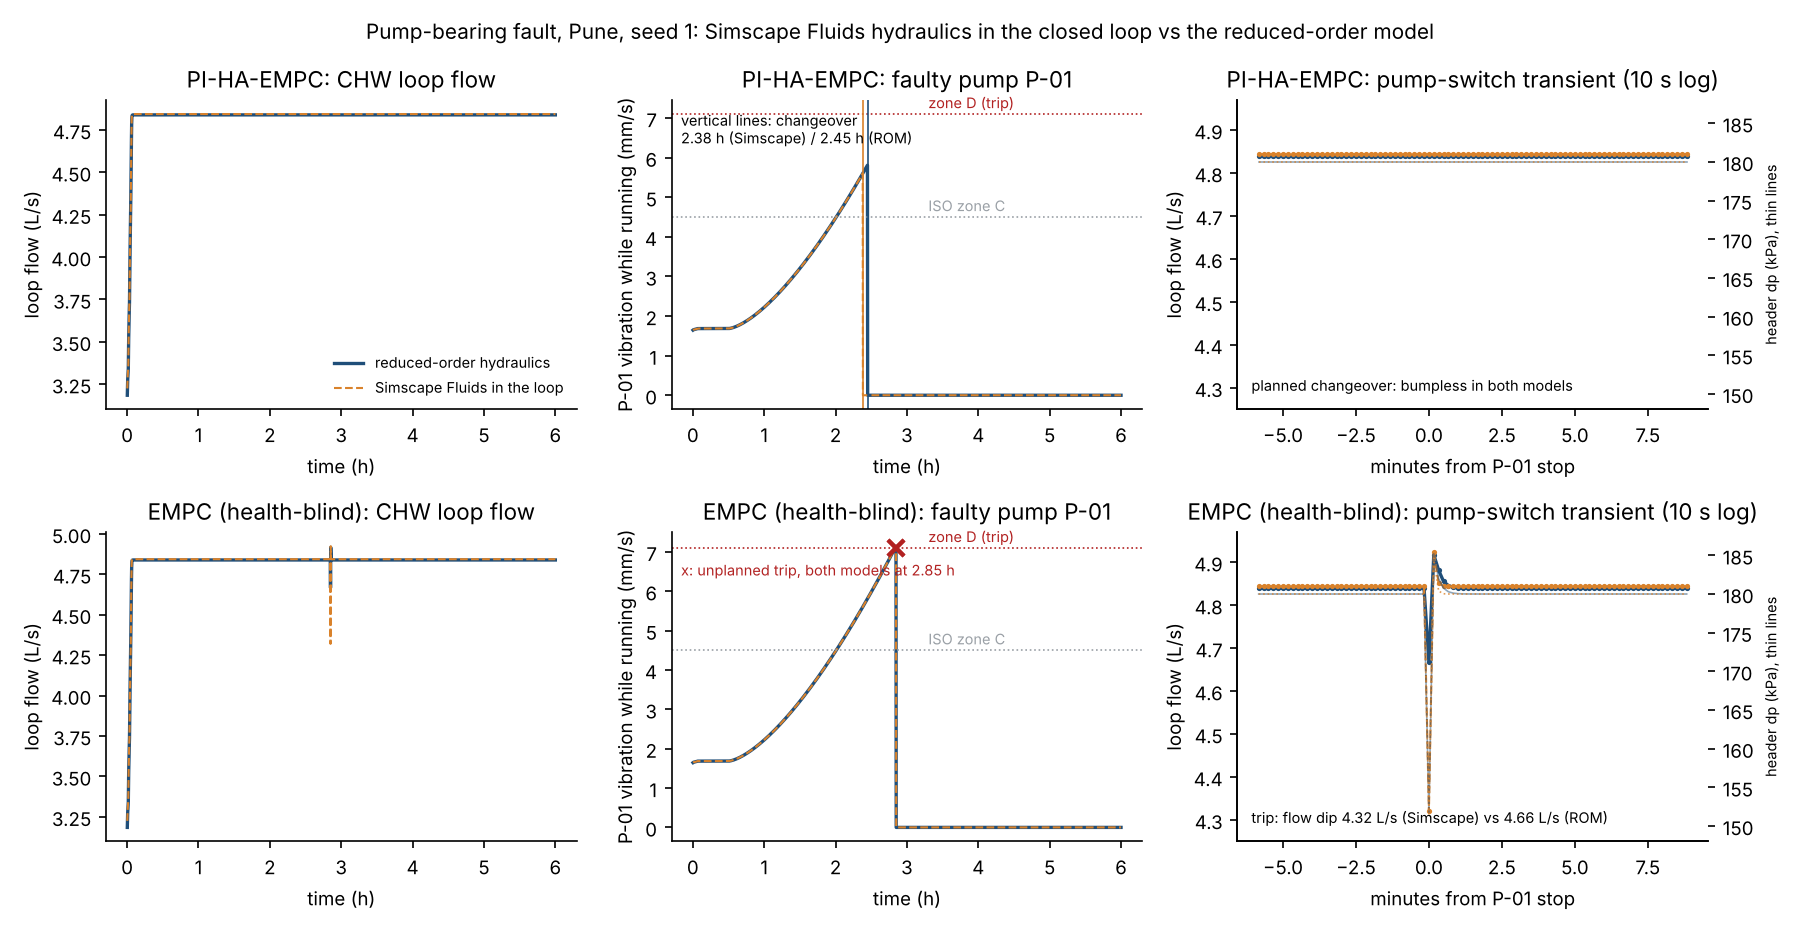
\includegraphics[width=\linewidth]{fig_ssc_loop}
\caption{Simscape Fluids CHW hydraulics in the closed loop against the reduced-order model (pump-bearing fault, Pune, seed 1). Left: loop flow. Centre: vibration of the faulty pump while running, with changeover (top) and unplanned trip (bottom). Right: flow (thick) and header DP (thin) around the pump switch.}\label{fig:sscloop}
\end{figure}
\paragraph{Energy balance} \Cref{tab:balance} reports the energy-balance closure over 4\,h of quasi-steady operation in both climates. The CHW-loop, condenser and metered-energy balances close to within numerical precision, and the electrical sum closes exactly. The room-air balance shows a residual of \CredRoomRaw\,\% of IT heat. We traced this to a modelling simplification: rack-inlet recirculation is represented by blending hot-aisle temperature into the inlet, without removing that air from the hot-aisle balance. The resulting enthalpy term, equal to \CredRecircPct\,\% of coil duty, overstates coil load. With this term included the room balance closes to within \CredRoomClosed\,\%. The overstatement applies equally to every controller, so it biases absolute cooling energy rather than the comparisons.
\paragraph{Step responses} \Cref{fig:steps} shows the closed-loop response of the PI baseline (flat workload, constant ambient). Tracked setpoint steps settle to 2\,\% in \CredSettleChws\,min (CHW supply, 18$\to$20\,\textdegree C) and \CredSettleSat\,min (supply air, 22$\to$23\,\textdegree C). After a +20\,\% IT-load step, the regulated maximum inlet temperature deviates by at most \CredItPeakInlet\,K and returns within $\pm$0.1\,K in \CredItRecover\,min.
\paragraph{Calibration} \Cref{fig:calib} compares the chiller map with the ASHRAE ratings, shows the two weather years, and compares the reduced-order hydraulics with Simscape Fluids.
\paragraph{Scope} All results are from simulation of a hypothetical facility. Component parameters are calibrated to code-minimum ratings and measured weather, not to a specific installed plant; degradation is time-compressed; and the plant model is reduced-order. The results establish relative performance under a verified model, not field savings.

\begin{table}[t]\centering\small
\caption{Energy-balance closure (mean residual over hours 2--6).}\label{tab:balance}
\begin{adjustbox}{max width=\linewidth}\begin{tabular}{lrrrrrr}
\toprule
Climate & Room air, raw (\%) & Recirculation term (\% of coil) & Room air, closed (\%) & CHW loop (\%) & Condenser (\%) & Energy meter (\%)\\
\midrule
Pune & -9.15 & 8.57 & -0.01 & 0.006 & 0.000 & -0.0045\\
Frankfurt & -9.15 & 8.55 & -0.01 & 0.007 & 0.000 & -0.0033\\
\bottomrule
\end{tabular}
\end{adjustbox}
\end{table}
\begin{figure}[t]\centering
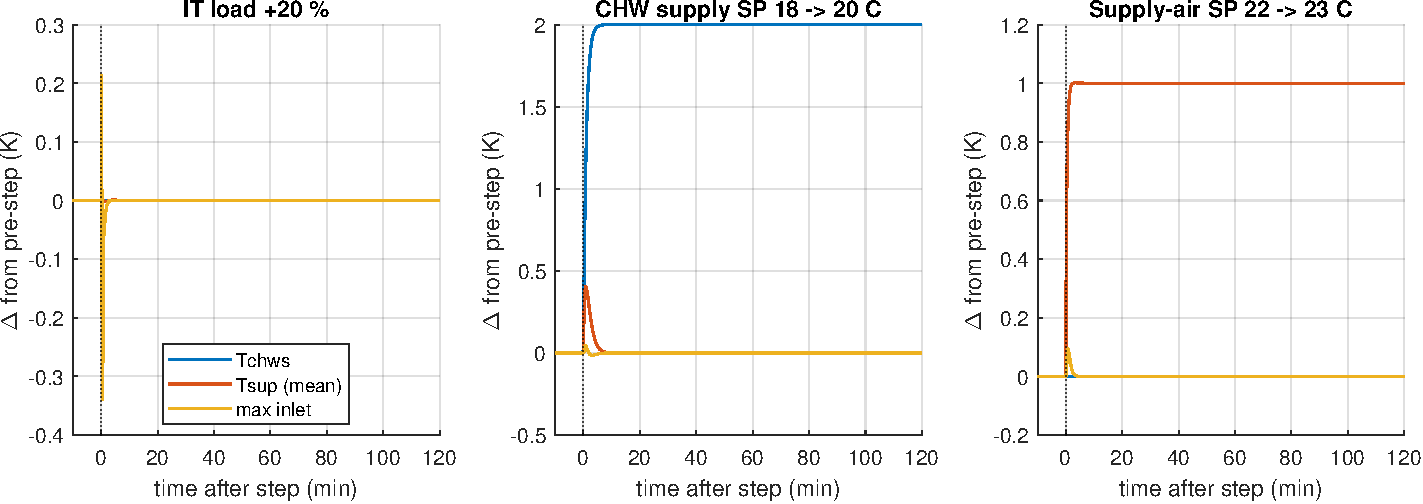
\includegraphics[width=\linewidth]{fig_step_responses}
\caption{Closed-loop step responses of the PI baseline (calibrated plant, constant ambient).}\label{fig:steps}
\end{figure}
\begin{figure}[t]\centering
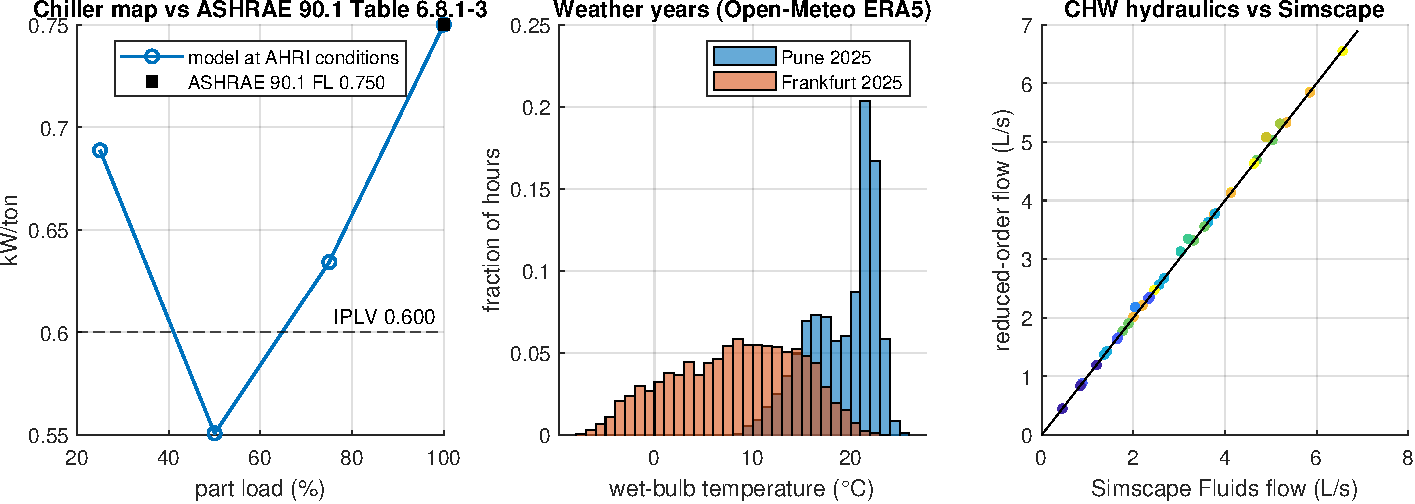
\includegraphics[width=\linewidth]{fig_calibration}
\caption{Calibration evidence: chiller map against ASHRAE 90.1 ratings, measured wet-bulb distributions, and CHW hydraulics against Simscape Fluids.}\label{fig:calib}
\end{figure}

%% =====================================================================
\section{Results}\label{sec:results}
\subsection{E1: energy and thermal performance}
\Cref{tab:E1} and \cref{fig:E1} summarise normal operation. Relative to fixed setpoints, PI-HA-EMPC changed cooling energy by \EoneCoolRelHaFixedPune\,\% [\EoneCoolRelHaFixedPuneLo, \EoneCoolRelHaFixedPuneHi] in Pune and \EoneCoolRelHaFixedFrankfurt\,\% [\EoneCoolRelHaFixedFrankfurtLo, \EoneCoolRelHaFixedFrankfurtHi] in Frankfurt, and facility energy by \EoneFacRelHaFixedPune\,\% and \EoneFacRelHaFixedFrankfurt\,\% respectively. Against health-blind EMPC the mean paired cooling-energy difference was $+0.003$\,\% (largest single-run difference 0.05\,\%). The difference is consistent in sign, so the signed-rank test detects it ($p\,\EoneCoolPHaEmpcAll$), but it is three orders of magnitude below the EMPC saving: without faults, health awareness costs essentially nothing. It arises because the move bounds scale with the lowest estimated HI, and measurement noise keeps that estimate slightly below 100 even for healthy equipment. No controller spent time above 28\,\textdegree C in any normal run.
\begin{table}[t]\centering\scriptsize
\caption{E1: normal operation, pooled over three workloads and ten seeds (mean [95\,\% CI]).}\label{tab:E1}
\begin{adjustbox}{max width=\linewidth}% generated by dcx_study_stats.m
\begin{tabular}{llrrrr}
\toprule
Climate & Controller & Facility energy (kWh) & Cooling energy (kWh) & PUE & Time $>$28\,\textdegree C (min)\\
\midrule
Pune & Baseline (fixed SP + PI) & 817.7 {\scriptsize[801.3, 834.2]} & 127.6 {\scriptsize[119.1, 136.0]} & 1.311 {\scriptsize[1.297, 1.324]} & 0.0 {\scriptsize[0.0, 0.0]}\\
 & EMPC & 791.6 {\scriptsize[775.2, 808.1]} & 101.6 {\scriptsize[92.9, 110.3]} & 1.269 {\scriptsize[1.255, 1.283]} & 0.0 {\scriptsize[0.0, 0.0]}\\
 & PI-HA-EMPC & 791.6 {\scriptsize[775.2, 808.1]} & 101.6 {\scriptsize[92.9, 110.3]} & 1.269 {\scriptsize[1.255, 1.283]} & 0.0 {\scriptsize[0.0, 0.0]}\\
\midrule
Frankfurt & Baseline (fixed SP + PI) & 754.0 {\scriptsize[738.6, 769.5]} & 64.2 {\scriptsize[57.8, 70.6]} & 1.208 {\scriptsize[1.199, 1.218]} & 0.0 {\scriptsize[0.0, 0.0]}\\
 & EMPC & 743.9 {\scriptsize[730.2, 757.6]} & 54.1 {\scriptsize[51.3, 56.9]} & 1.192 {\scriptsize[1.188, 1.197]} & 0.0 {\scriptsize[0.0, 0.0]}\\
 & PI-HA-EMPC & 743.9 {\scriptsize[730.2, 757.6]} & 54.1 {\scriptsize[51.3, 56.9]} & 1.192 {\scriptsize[1.188, 1.197]} & 0.0 {\scriptsize[0.0, 0.0]}\\
\bottomrule
\end{tabular}
\end{adjustbox}
\end{table}
\begin{figure}[t]\centering
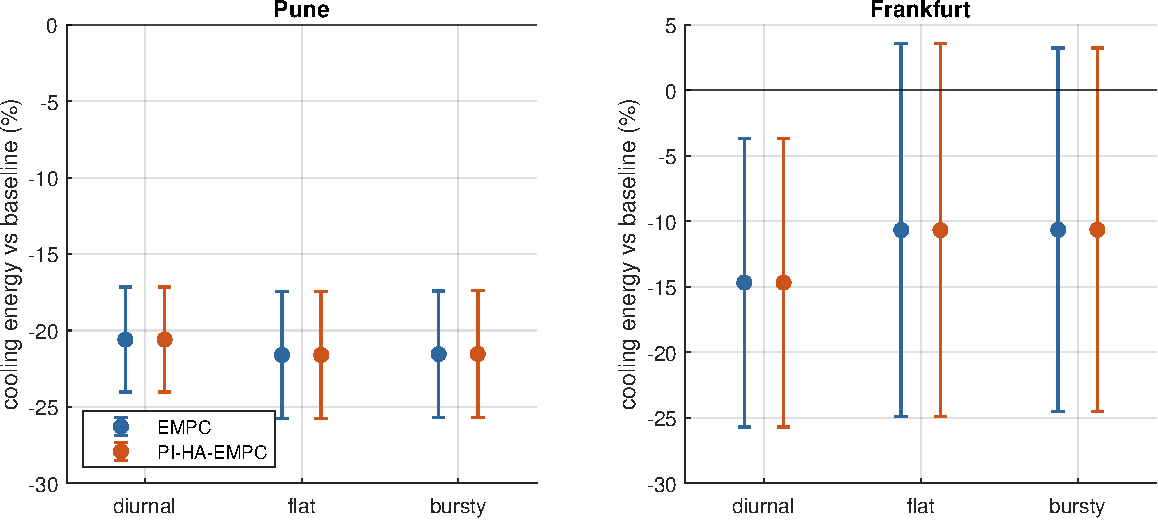
\includegraphics[width=\linewidth]{fig_E1_cooling_savings}
\caption{E1: paired cooling-energy change relative to the fixed-setpoint baseline per climate and workload (mean and 95\,\% CI over ten seeds).}\label{fig:E1}
\end{figure}

\subsection{E2: equipment risk under degradation}
\Cref{tab:E2} reports the fault scenarios. Fixed-setpoint control and EMPC cannot act on degradation they do not observe, so the protective trips occur while the asset is on duty (\EtwoTripsFixed{} and \EtwoTripsEmpc{} runs). PI-HA-EMPC changed over the pump or transferred the chiller lead beforehand, leaving \EtwoTripsHa{} unplanned trips (Wilson 95\,\% upper bound 0.09). Fewer than 40 baseline runs tripped because in Frankfurt the degrading chiller was often idle at the trip time, with the economiser carrying the load (\cref{sec:discussion}). PI-HA-EMPC also reduced zone-C/D exposure from \EtwoRiskEmpc\,min to \EtwoRiskHa\,min per pump-fault run. Facility energy in the fault runs differed from EMPC by less than 0.1\,\% (\cref{tab:E2}), so the avoided trips came at no measurable energy cost.
\begin{table}[t]\centering\scriptsize
\caption{E2: fault scenarios (trip rate with Wilson 95\,\% CI; other columns mean [95\,\% CI]).}\label{tab:E2}
\begin{adjustbox}{max width=\linewidth}% generated by dcx_study_stats.m
\begin{tabular}{lllrrr}
\toprule
Fault & Climate & Controller & Unplanned trips (rate) & Zone C/D exposure (min) & Energy (kWh)\\
\midrule
Chiller & Pune & Baseline (fixed SP + PI) & 10/10 {\scriptsize[0.72, 1.00]} & 0.0 {\scriptsize[0.0, 0.0]} & 871.6 {\scriptsize[851.5, 891.7]}\\
 &  & EMPC & 10/10 {\scriptsize[0.72, 1.00]} & 0.0 {\scriptsize[0.0, 0.0]} & 843.1 {\scriptsize[823.0, 863.1]}\\
 &  & PI-HA-EMPC & 0/10 {\scriptsize[0.00, 0.28]} & 0.0 {\scriptsize[0.0, 0.0]} & 842.2 {\scriptsize[822.5, 862.0]}\\
 & Frankfurt & Baseline (fixed SP + PI) & 7/10 {\scriptsize[0.40, 0.89]} & 0.0 {\scriptsize[0.0, 0.0]} & 804.7 {\scriptsize[787.4, 822.0]}\\
 &  & EMPC & 4/10 {\scriptsize[0.17, 0.69]} & 0.0 {\scriptsize[0.0, 0.0]} & 791.3 {\scriptsize[779.8, 802.8]}\\
 &  & PI-HA-EMPC & 0/10 {\scriptsize[0.00, 0.28]} & 0.0 {\scriptsize[0.0, 0.0]} & 791.2 {\scriptsize[779.8, 802.7]}\\
\midrule
Pump & Pune & Baseline (fixed SP + PI) & 10/10 {\scriptsize[0.72, 1.00]} & 49.8 {\scriptsize[49.8, 49.8]} & 867.2 {\scriptsize[847.9, 886.5]}\\
 &  & EMPC & 10/10 {\scriptsize[0.72, 1.00]} & 50.3 {\scriptsize[50.3, 50.3]} & 840.9 {\scriptsize[821.5, 860.2]}\\
 &  & PI-HA-EMPC & 0/10 {\scriptsize[0.00, 0.28]} & 24.5 {\scriptsize[23.1, 26.0]} & 840.8 {\scriptsize[821.5, 860.2]}\\
 & Frankfurt & Baseline (fixed SP + PI) & 10/10 {\scriptsize[0.72, 1.00]} & 49.7 {\scriptsize[49.6, 49.8]} & 803.2 {\scriptsize[786.7, 819.7]}\\
 &  & EMPC & 10/10 {\scriptsize[0.72, 1.00]} & 50.2 {\scriptsize[50.0, 50.4]} & 791.2 {\scriptsize[779.8, 802.5]}\\
 &  & PI-HA-EMPC & 0/10 {\scriptsize[0.00, 0.28]} & 24.4 {\scriptsize[23.0, 25.8]} & 791.2 {\scriptsize[779.8, 802.5]}\\
\bottomrule
\end{tabular}
\end{adjustbox}
\end{table}

\subsection{E3: ablations}
\begin{table}[t]\centering\scriptsize
\caption{E3: ablations over both fault scenarios and climates (diurnal workload).}\label{tab:E3}
\begin{adjustbox}{max width=\linewidth}% generated by dcx_study_stats.m; E3b rows added from runs_ablation2.csv (same statistics, abl2.py)
\begin{tabular}{lrrrr}
\toprule
Variant & Unplanned trips & Zone C/D exposure (min) & Peak inlet (\textdegree C) & Energy (kWh)\\
\midrule
PI-HA-EMPC (full) & 0/40 {\scriptsize[0.00, 0.09]} & 12.2 {\scriptsize[8.2, 16.2]} & 26.60 {\scriptsize[26.59, 26.60]} & 816.4 {\scriptsize[805.7, 827.0]}\\
without Health Index & 3/40 {\scriptsize[0.03, 0.20]} & 17.4 {\scriptsize[11.7, 23.1]} & 26.62 {\scriptsize[26.61, 26.62]} & 816.9 {\scriptsize[806.1, 827.6]}\\
without RUL & 1/40 {\scriptsize[0.00, 0.13]} & 12.2 {\scriptsize[8.2, 16.2]} & 26.60 {\scriptsize[26.59, 26.60]} & 816.4 {\scriptsize[805.7, 827.0]}\\
without pre-cooling & 1/40 {\scriptsize[0.00, 0.13]} & 12.2 {\scriptsize[8.2, 16.2]} & 26.60 {\scriptsize[26.59, 26.60]} & 816.4 {\scriptsize[805.7, 827.0]}\\
\midrule
\multicolumn{5}{l}{\textit{Component ablations (E3b)}}\\
health in the MPC only (no discrete actions) & 34/40 {\scriptsize[0.71, 0.93]} & 25.1 {\scriptsize[17.0, 33.3]} & 26.63 {\scriptsize[26.59, 26.66]} & 818.2 {\scriptsize[807.3, 829.1]}\\
discrete actions only (health-blind MPC) & 0/40 {\scriptsize[0.00, 0.09]} & 12.2 {\scriptsize[8.2, 16.2]} & 26.60 {\scriptsize[26.59, 26.61]} & 816.3 {\scriptsize[805.7, 827.0]}\\
\midrule
EMPC (no health information) & 34/40 {\scriptsize[0.71, 0.93]} & 25.1 {\scriptsize[17.0, 33.3]} & 26.67 {\scriptsize[26.60, 26.75]} & 816.6 {\scriptsize[805.9, 827.4]}\\
\bottomrule
\end{tabular}
\end{adjustbox}
\end{table}
\Cref{tab:E3} isolates each mechanism. No ablated variant produced an unplanned pump trip, and in Pune none produced a chiller trip, because the HI and RUL triggers are redundant: removing one leaves the other to fire. The ordering of the triggers still matters. Without the HI trigger the pump changeover waits for the RUL window, so zone-C/D exposure rose from about 1470\,s to about 2090\,s per pump-fault run in both climates. In the Frankfurt chiller scenario the full PI-HA-EMPC avoided every trip, whereas the no-HI variant tripped in 3 of 10 seeds and the no-RUL and no-pre-cooling variants in 1 of 10. That one case (seed 4) was the only marginal one. Without RUL the HI threshold was not crossed in time. Without pre-cooling the lead transfer completed, but the degraded unit was still on duty when it tripped (see E3b for the cause). Elsewhere pre-cooling changed neither trips nor exposure, and it changed facility energy by less than 0.1\,\%.

\paragraph{E3b: MPC-side health versus discrete actions} Two further variants separate the two places health enters the controller (\cref{tab:E3}, lower block; \cref{fig:E3b}). With health used only inside the MPC (HI-scaled move bounds and pre-cooling, no changeover or lead transfer), the trip rate was the same as health-blind EMPC: 34 of 40 runs, the same runs. Facility energy was 0.2\,\% higher (at most 0.6\,\% in a paired run) because of pre-cooling. With the discrete actions alone on a health-blind MPC, no run tripped. Exposure and energy matched the full controller (paired energy within 0.02\,\%). This holds in the Frankfurt seed-4 case as well. There the no-pre-cooling variant tripped while the actions-only variant did not, so the trip was caused by the HI-scaled move bounds acting without pre-cooling, not by a missing mechanism. A sanity variant with every health input switched off reproduced EMPC exactly (6 paired runs, identical energy, temperatures and trips). In these scenarios, therefore, all of the trip avoidance comes from the health-triggered supervisory actions. The MPC-side terms gave no protection and, in the one marginal case, interacted badly with the sequencing.
\begin{figure}[t]\centering
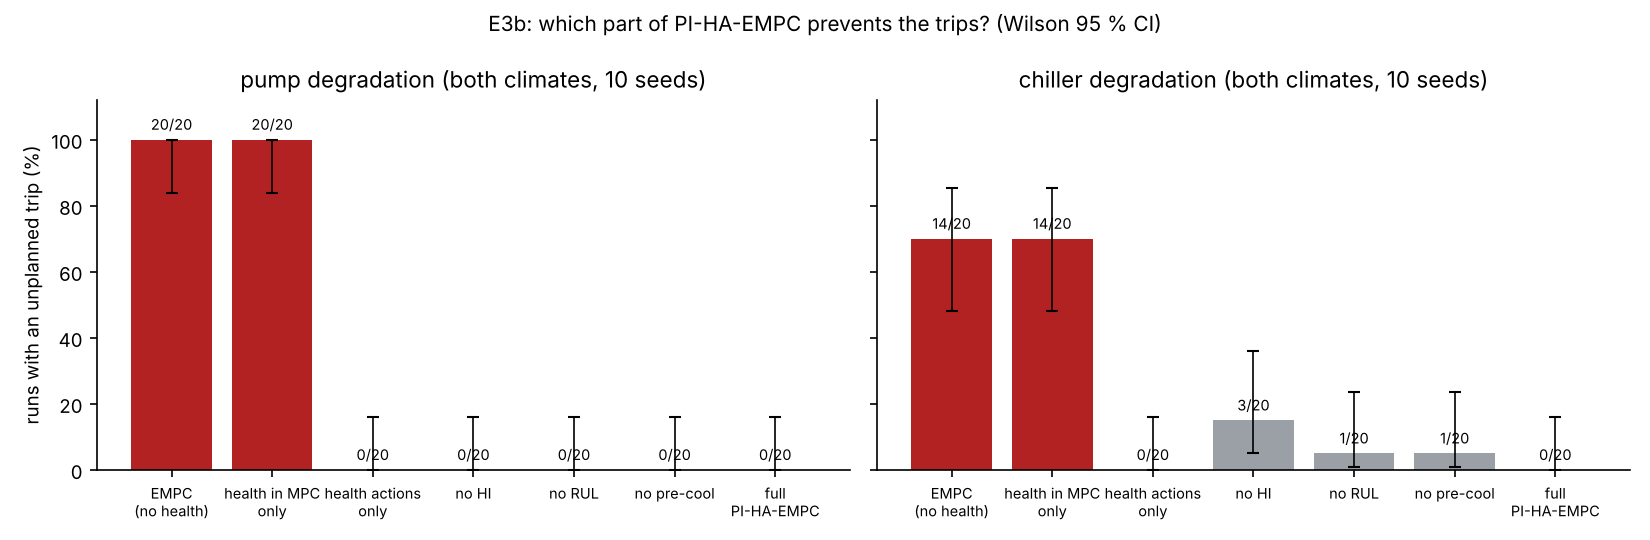
\includegraphics[width=\linewidth]{fig_E3b_components}
\caption{E3b: unplanned-trip rate when health is used only inside the MPC, only through the discrete actions, or both (both climates, ten seeds, diurnal workload; Wilson 95\,\% CI).}\label{fig:E3b}
\end{figure}

\subsection{E4: sensitivity to RUL estimation error}
\begin{table}[t]\centering\scriptsize
\caption{E4: RUL estimation error (estimate multiplied by the scale factor; Pune, diurnal).}\label{tab:E4}
\begin{adjustbox}{max width=\linewidth}% generated by dcx_study_stats.m
\begin{tabular}{lrrrr}
\toprule
Fault & RUL error & Unplanned-trip rate & Zone C/D exposure (min) & Pre-cooling (min)\\
\midrule
Chiller & -50\,\% & 0.00 {\scriptsize[0.00, 0.28]} & 0.0 {\scriptsize[0.0, 0.0]} & 4 {\scriptsize[3, 4]}\\
 & +0\,\% & 0.00 {\scriptsize[0.00, 0.28]} & 0.0 {\scriptsize[0.0, 0.0]} & 4 {\scriptsize[3, 4]}\\
 & +50\,\% & 0.00 {\scriptsize[0.00, 0.28]} & 0.0 {\scriptsize[0.0, 0.0]} & 4 {\scriptsize[3, 5]}\\
 & +100\,\% & 0.00 {\scriptsize[0.00, 0.28]} & 0.0 {\scriptsize[0.0, 0.0]} & 4 {\scriptsize[3, 5]}\\
 & +200\,\% & 0.00 {\scriptsize[0.00, 0.28]} & 0.0 {\scriptsize[0.0, 0.0]} & 4 {\scriptsize[3, 5]}\\
\midrule
Pump & -50\,\% & 0.00 {\scriptsize[0.00, 0.28]} & 21.3 {\scriptsize[19.1, 23.6]} & 17 {\scriptsize[13, 20]}\\
 & +0\,\% & 0.00 {\scriptsize[0.00, 0.28]} & 24.5 {\scriptsize[23.1, 26.0]} & 1 {\scriptsize[0, 1]}\\
 & +50\,\% & 0.00 {\scriptsize[0.00, 0.28]} & 24.5 {\scriptsize[23.1, 26.0]} & 0 {\scriptsize[0, 0]}\\
 & +100\,\% & 0.00 {\scriptsize[0.00, 0.28]} & 24.5 {\scriptsize[23.1, 26.0]} & 0 {\scriptsize[0, 0]}\\
 & +200\,\% & 0.00 {\scriptsize[0.00, 0.28]} & 24.5 {\scriptsize[23.1, 26.0]} & 0 {\scriptsize[0, 0]}\\
\bottomrule
\end{tabular}
\end{adjustbox}
\end{table}
\begin{figure}[t]\centering
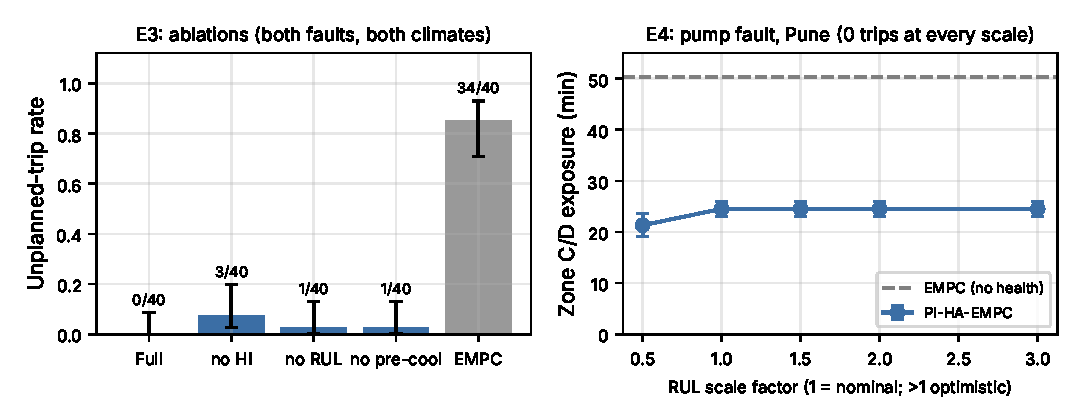
\includegraphics[width=\linewidth]{fig_E3E4_risk}
\caption{Left: unplanned-trip rate by ablation variant (Wilson 95\,\% CI). Right: zone-C/D exposure in the pump-fault runs against the RUL scale factor (mean and 95\,\% CI over ten seeds); no run tripped at any scale.}\label{fig:E34}
\end{figure}
Because the HI trigger is unaffected by RUL scaling, optimistic RUL errors ($1.5$--$3\times$) produced exactly the nominal behaviour: no trips and the same exposure (\cref{tab:E4}). A pessimistic error ($0.5\times$) brought the pump changeover forward, lowering exposure from about 1470\,s to 1280\,s at the cost of about 17\,min of extra pre-cooling, and had no effect in the chiller scenario. Within the tested range, the scheme's tolerance to RUL error comes from the redundant HI trigger rather than from the accuracy of the prognosis.

\subsection{E5: diagnosis and prognosis accuracy}
\Cref{tab:E5} reports held-out diagnosis accuracy (split by run, 120 runs, 12 classes), with 95\,\% intervals from a cluster bootstrap over test runs. Adding physics-residual features raised macro-F1 most for the plant faults (chiller, heat exchanger and towers): from \EfivePlantSensor{} to \EfivePlant{} [\EfivePlantLo, \EfivePlantHi]. The control loops mask these faults' raw sensor signatures. For pump-bearing RUL on \EfiveRulRuns{} held-out run-to-failure runs, the exponential degradation model gave an RMSE of \EfiveRulRmse\,min [\EfiveRulRmseLo, \EfiveRulRmseHi] (\EfiveRulLate\,min over the last half of life), with 90\,\% interval coverage of \EfiveRulCover. The small number of run-to-failure runs makes the RUL interval wide; this is one motivation for the error-sensitivity analysis in E4. Degradation is time-compressed.
\begin{table}[t]\centering\small
\caption{E5: diagnosis macro-F1 on held-out runs (cluster-bootstrap 95\,\% CI).}\label{tab:E5}
\begin{adjustbox}{max width=\linewidth}% generated by dcx_e5_ci.m
\begin{tabular}{lrr}
\toprule
Asset class & Sensor-only macro-F1 & Sensor + physics-residual macro-F1\\
\midrule
CHW pumps & 0.993 {\scriptsize[0.988, 1.000]} & 1.000 {\scriptsize[1.000, 1.000]}\\
CRAH fans & 0.955 {\scriptsize[0.891, 0.995]} & 0.983 {\scriptsize[0.931, 1.000]}\\
Chiller / HX / towers & 0.608 {\scriptsize[0.471, 0.815]} & 0.988 {\scriptsize[0.979, 1.000]}\\
\bottomrule
\end{tabular}
\end{adjustbox}
\end{table}

\subsection{E6: computational cost}
\begin{table}[t]\centering\small
\caption{E6: \texttt{mpcmove} wall time per 60\,s supervisory step (MATLAB R2024a, laptop CPU).}\label{tab:E6}
\begin{adjustbox}{max width=\linewidth}% generated by dcx_study_stats.m
\begin{tabular}{lrrrr}
\toprule
Controller & MPC solves & Mean (ms) & Median per-run p95 (ms) & Max (ms)\\
\midrule
empc & 36000 & 25.1 & 32.0 & 902.7\\
ha\_noHI & 14400 & 25.0 & 32.1 & 110.0\\
ha\_noPrecool & 14400 & 24.8 & 32.2 & 77.6\\
ha\_noRUL & 14400 & 24.8 & 32.2 & 69.5\\
haempc & 64800 & 24.5 & 32.5 & 466.7\\
\bottomrule
\end{tabular}
\end{adjustbox}
\end{table}
The mean solve time was \EsixMeanMs\,ms and the worst case \EsixMaxMs\,ms (a single outlier; per-run 95th percentiles were about 32\,ms), so even the worst case is about 60 times shorter than the 60\,s sampling period (\cref{tab:E6}). The health logic adds negligible cost.

%% =====================================================================
\section{Discussion}\label{sec:discussion}
\paragraph{Where health awareness pays} In healthy operation PI-HA-EMPC behaves like EMPC, so its energy benefit over thermostatic control is that of EMPC. Its value appears under degradation: it turns forced, on-duty trips into planned changeovers taken while thermal margin still exists. Because these actions are discrete and cheap, avoiding the trips costs no measurable energy. E3b sharpens this: the protection comes from the health-triggered supervisory layer around the EMPC, not from health terms inside the optimisation. A simpler design, health-blind EMPC with health-triggered changeover and lead transfer, matched the full controller here. Health-aware constraints inside the MPC may still pay off in faults that cannot be handled by switching to a standby unit (no redundancy, or common-mode degradation), which these scenarios did not include. This complements the implementability-gap view of \citet{Jadhav2026DT}: equipment condition is a further constraint on deployable control, and it is better exploited than ignored.
\paragraph{Prognostic accuracy as a design input} E3 and E4 together suggest that a condition threshold and a prognostic window should be used side by side. Pessimistic RUL estimates cost only earlier changeovers and longer pre-cooling, and optimistic ones were absorbed by the HI threshold. The RUL channel is not idle: it is the only trigger that remains if the HI thresholds are tuned too loosely, as the no-HI variant shows.
\paragraph{Observability depends on load} In Frankfurt the economiser carries most of the load for much of the year, so at the scheduled trip time the degrading chiller was often idle. An idle chiller produces no COP residual, so its HI is not updated, and the trip of an idle asset is not unplanned. This explains the lower trip rates of all controllers in Frankfurt, and it means that health-aware schemes should schedule periodic proving runs for standby or seasonally idle equipment.
\paragraph{A sequencing defect found by the study} In an earlier version of the supervisor, the chiller pre-start and lead transfer were evaluated on the instantaneous trigger. In one Frankfurt seed the trigger dropped out after the pre-start, so the lead transfer never happened and the chiller tripped on duty. We latched the sequence (once pre-started, the transfer always follows after 240\,s) and reran every affected run; all reported results use the latched supervisor, and the pre-fix results are kept in the released data. Such defects in discrete logic are invisible in average energy metrics, which is a further argument for multi-seed evaluation.
\paragraph{Limitations} (i) The plant is reduced-order and simulated; the Simscape Fluids co-simulation covers the CHW hydraulics only, in one scenario, and the thermal plant remains reduced-order; field savings depend on the installed equipment, sensors and baseline. (ii) Faults and their protective thresholds are modelled, and degradation is time-compressed into hours. (iii) The prediction model is linear and identified per climate; its power fit is lower in Frankfurt (55\,\%) because economiser switching is strongly nonlinear, and the 0.2\,K back-off covers the inlet-model error only empirically. (iv) A single 8-rack facility is studied. (v) The generator's emissions are not included in CO$_2$. (vi) Rack-inlet recirculation is not energy-conserving in the air model (\cref{sec:cred}); it overstates coil load by about \CredRecircPct\,\% for all controllers alike.
\paragraph{Path to deployment} The supervisor runs on 60\,s supervisory setpoints and standard plant commands, which are exactly the interface exposed by building-management and SCADA systems. Our testbed exercises this through OPC~UA and Ignition, which makes a hardware-in-the-loop or shadow-mode trial the natural next step.

%% =====================================================================
\section{Conclusions}\label{sec:conclusion}
We formulated a health-aware economic MPC for data-centre cooling that uses live Health Index and RUL estimates. On a calibrated, cross-verified simulation twin evaluated across two climates, three workloads and ten seeds, it matched health-blind EMPC in energy and avoided unplanned cooling-equipment trips under degradation. Ablations attributed the benefit to the health-triggered supervisory actions, with the RUL trigger as a backstop to the HI trigger. Health terms inside the MPC added no trip protection in these scenarios. The redundancy between the triggers made the scheme insensitive to optimistic RUL errors up to $3\times$ in the scenarios studied. All results are from simulation; the code, configuration and seeds are released for reproduction.

\section*{Data and code availability}
All code (MATLAB/Simulink models, controllers, experiment scripts), configuration files, random seeds and the generated result tables are available at \url{https://doi.org/10.5281/zenodo.XXXXXXX} (frozen release v1.0.0). Weather data are from the Open-Meteo historical archive (ERA5-based) and are downloaded by the provided scripts. No proprietary or personal data were used.

\section*{CRediT authorship contribution statement}
\textbf{Anup Deshmukh}: Conceptualization, Methodology, Software, Validation, Formal analysis, Investigation, Writing -- original draft, Writing -- review \& editing, Visualization.

\section*{Declaration of competing interest}
The author declares no known competing financial interests or personal relationships that could have appeared to influence the work reported in this paper.

\section*{Declaration of generative AI and AI-assisted technologies in the writing process}
During the preparation of this work the author used Claude (Anthropic) to draft and refactor code, scripts and text. After using this tool, the author reviewed and edited the content as needed and takes full responsibility for the content of the publication. All reported results were produced by running the released code.

\bibliographystyle{elsarticle-harv}
\bibliography{refs}
\end{document}
